\chapter[The Affine Structure: Drift and Control]{The Affine Structure:\\Drift and Control}
\raggedbottom
\label{ch:05_affine_structure}
\index{control-affine}\index{control-affine form}\index{integral curve}\index{orbit}

\begin{laymansbox}{The Big Reveal}{box:ch05_big_reveal}
A swing combines energy supplied by muscles with motion shaped by inertia, gravity, contact and tissue mechanics. The control-affine description makes one part of this interaction explicit: at a fixed state, how does a chosen input change the state derivative? It is a useful mathematical structure, not proof that skilled movement is predominantly passive.

For an ideal unconstrained rigid model in local coordinates,
\begin{equation}
 M(q)\ddot q+c(q,\dot q)+g(q)=B(q)u.
\label{eq:ch05_manipulator_repeat}
\end{equation}
The same model can be written
\begin{equation}
 \dot x=f(x)+G(x)u.
\label{eq:ch05_affine_repeat}
\end{equation}
The meaning of zero input, the admissible inputs and the retained state must accompany this equation. It does not decide which part of the swing supplies energy, which control is optimal, or how the nervous system implements a policy. Those questions require additional calculations and evidence.
\end{laymansbox}

\section{From Equations of Motion to State Space}
\subsection*{Defining State}
For $n$ independent local joint coordinates, write $v=\dot q$ and
\begin{equation}
 x=\begin{bmatrix}q\\v\end{bmatrix}\in\mathbb R^{2n}.
\label{eq:ch05_state_def}
\end{equation}
A two-joint planar example has $x=(q_1,q_2,v_1,v_2)^T$. This is a local chart, not a complete human description or a globally unique representation of periodic angles. A general rigid-body implementation may instead use $\dot q=N(q)v$, with different position and velocity dimensions. Activation, flexible tissues and shaft deformation require their own state variables.

\begin{equation}
 \dot x=\begin{bmatrix}v\\\dot v\end{bmatrix}.
\label{eq:ch05_state_derivative}
\end{equation}
A zero velocity at one instant is not a zero acceleration. The top block describes the rate of position change; the lower block determines how velocity changes.

\subsection*{Solving for Accelerations}
Assume $M$ is symmetric positive definite on the independent coordinates. Define $c$ as the complete velocity-dependent inertial bias, and $g=\nabla_q V$ for the gravitational potential. A matrix $C$ may satisfy $c=Cv$, but that factorization is not unique; dropping selected entries without deriving their product changes the dynamics. The standard manipulator formulation and its coordinate limitations are developed in \citep{TedrakeMultibodyEnergy}.
\begin{equation}
 \dot v=M^{-1}(Bu-c-g).
\label{eq:ch05_solve_accel}
\end{equation}
Numerically, solve the mass-matrix system rather than explicitly forming its inverse. The inverse notation is useful for analysis:
\begin{equation}
 \dot v=\underbrace{-M^{-1}(c+g)}_{a_0(q,v)}+
          \underbrace{M^{-1}Bu}_{a_u(q,v,u)}.
\label{eq:ch05_accel_decomposed}
\end{equation}
Additional declared passive generalized forces belong in the corresponding bias; a moving base or contact introduces further terms or constraints.

\subsection*{The Control-Affine Form}
\begin{equation}
 f(x)=\begin{bmatrix}v\\a_0\end{bmatrix},\qquad
 G(x)=\begin{bmatrix}0_{n\times m}\\M^{-1}B\end{bmatrix},\qquad
 \dot x=f(x)+G(x)u.
\label{eq:ch05_control_affine_form}
\end{equation}
Drift contains the kinematic block $v$ as well as the uncontrolled acceleration. The zero position block of $G$ means torque changes acceleration immediately in this ideal model; later position changes follow through integration. It does not mean position is uncontrollable over time.

\begin{definition}{Control-Affine Systems}{ch05_control_affine}
At each fixed state, an affine input map has a constant offset and a linear part:
\begin{equation}
 F(x,u)=f(x)+G(x)u.
\label{eq:ch05_control_affine_def}
\end{equation}
Its state dependence may be nonlinear or linear. The linear system $\dot x=Ax+Bu$ is also control-affine, with $f=Ax$. An affine combination of two inputs produces the corresponding affine combination of derivatives at the same state; this does not imply superposition of complete nonlinear trajectories. Nonzero $f$ means the input-to-derivative map is generally not a homogeneous linear map.
\end{definition}

\begin{laymansbox}{Why Affine Matters}{box:ch05_why_affine}
The columns of $G$ describe local directions available through the chosen inputs. The set $f+G\mathcal U$ describes attainable derivatives when inputs lie in $\mathcal U$. This separates the local mechanics from the problem of selecting an input for a particular goal. Torque limits, muscle redundancy and delayed activation make $\mathcal U$ and its evolution as important as the matrix itself.

Here $u$ is generalized actuator torque. It is not automatically muscle excitation. Two muscle patterns can yield the same net joint torque but different stiffness, metabolic cost and future force capacity. Defining zero torque therefore does not identify a relaxed muscle state.
\end{laymansbox}

\section{Explicit Form for the Double Pendulum}
Define two rigid links joined by ideal planar hinges, with the proximal pivot fixed. Let $q_1$ measure the first link from downward vertical and $q_2$ the second link relative to the first, so its absolute angle is $q_1+q_2$. Link masses are $m_i$, proximal-to-COM distances $r_i$, first-link length $l_1$, and COM inertias $I_i$. Torques $u_1,u_2$ are conjugate to these relative coordinates; $B=I$. This idealization retains coupling but does not resolve anatomical wrist planes, both arms or a flexible club.

Set
\[
 A=I_1+m_1r_1^2+m_2l_1^2,\qquad D=I_2+m_2r_2^2,\qquad b=m_2l_1r_2.
\]
The COM positions are $p_1=r_1(\sin q_1,-\cos q_1)^T$ and $p_2=l_1(\sin q_1,-\cos q_1)^T+r_2(\sin(q_1+q_2),-\cos(q_1+q_2))^T$. Their translational energies and the absolute angular rates $v_1,v_1+v_2$ give
\[
 M=\begin{bmatrix}A+D+2b\cos q_2&D+b\cos q_2\\D+b\cos q_2&D\end{bmatrix},
 \qquad T=\tfrac12 v^TMv.
\]
The potential and complete bias are
\[
 \begin{aligned}
 V&=-g_0\big[(m_1r_1+m_2l_1)\cos q_1+m_2r_2\cos(q_1+q_2)\big],\\
 c&=b\sin q_2\begin{bmatrix}-2v_1v_2-v_2^2\\v_1^2\end{bmatrix},\\
 g&=g_0\begin{bmatrix}(m_1r_1+m_2l_1)\sin q_1+m_2r_2\sin(q_1+q_2)\\m_2r_2\sin(q_1+q_2)\end{bmatrix}.
 \end{aligned}
\]
Here $g_0$ is gravitational acceleration, while $g$ is a generalized-force vector. The second bias component can be nonzero when $v_2=0$; a rotating first link still affects the second. All inertias are about the COM, avoiding double-counting parallel-axis terms.

\subsection*{The Drift Vector Field}
With $h=c+g$ and $K=M^{-1}$,
\begin{equation}
 f(x)=\begin{bmatrix}v_1\\v_2\\-K_{11}h_1-K_{12}h_2\\-K_{21}h_1-K_{22}h_2\end{bmatrix}.
\label{eq:ch05_drift_vector}
\end{equation}
Both bias components enter each acceleration through inverse inertia. Dependence on the current state does not erase the effect of prior control: earlier torques helped create that state.

\subsection*{The Control Matrix}
\begin{equation}
 G=\begin{bmatrix}0&0\\0&0\\K_{11}&K_{12}\\K_{21}&K_{22}\end{bmatrix}.
\label{eq:ch05_control_matrix}
\end{equation}
\begin{equation}
 u=(u_1,u_2)^T.
\label{eq:ch05_control_input}
\end{equation}
\begin{equation}
 (\dot q_1,\dot q_2,\dot v_1,\dot v_2)^T=f(x)+G(x)u.
\label{eq:ch05_full_affine}
\end{equation}
The off-diagonal entries express coupled acceleration. They do not assign the net joint torque to a unique muscle or determine the club's Cartesian acceleration without kinematics.

\begin{example}{Drift in the Double Pendulum at Rest}{ch05_drift_at_rest}
Use manufactured parameters $m_1=2.5$ kg, $m_2=0.4$ kg, $l_1=0.35$ m, $r_1=0.175$ m, $r_2=0.5$ m, $I_1=0.025$ and $I_2=0.030$ kg m$^2$, and $g_0=9.81$ m/s$^2$. They are a declared calculation, not fitted golfer data.

At $q=(0,0)$ and $v=0$, both gravity torques vanish, so $f=0$. The vertical downward configuration is a modeled equilibrium, not every golfer's address posture. At $q=(45^\circ,0)$ and $v=0$,
\[
 \begin{aligned}
 M&=\begin{bmatrix}0.4205625&0.2\\0.2&0.13\end{bmatrix}\ \mathrm{kg\,m^2},\\
 g&\simeq\begin{bmatrix}5.3933\\1.3873\end{bmatrix}\ \mathrm{N\,m},\qquad
 a_0\simeq\begin{bmatrix}-28.8732\\33.7484\end{bmatrix}\ \mathrm{rad/s^2}.
 \end{aligned}
\]
The relative second-joint acceleration is positive even though gravity draws the total system toward lower potential. It cannot be calculated from the first gravity component and $K_{11}$ alone. An inverse inertia has units $(\mathrm{kg\,m^2})^{-1}$; angular units should accompany reported rates.
\end{example}

\section{Drift as a Vector Field}
\begin{definition}{Vector Field}{ch05_vector_field}
A state vector field assigns a tangent vector to each state. Its integral curves satisfy the differential equation at every time. A drawn path through some arrows is not necessarily such a curve. A projection of a four-dimensional trajectory can be displayed in two coordinates, but its apparent derivative may also depend on the hidden coordinates.
\end{definition}

\begin{laymansbox}{What Is a Vector Field?}{box:ch05_vector_field}
A two-dimensional slice of a double-pendulum state space is not generally invariant: the trajectory can leave it immediately. To obtain a genuine two-state example, impose the ideal stationary constraint $q_2=0$, $v_2=0$. Its reaction maintains the lock and performs zero work. With zero proximal torque, the reduced equation is
\[
 (A+D+2b)\ddot q_1+g_0(m_1r_1+m_2l_1+m_2r_2)\sin q_1=0.
\]
The figure integrates this equation from $(q_1,v_1)=(0.9,0)$. This is drift of a different, constrained effective plant; it is not the free two-joint system with both torques set to zero. Arrow lengths are normalized for visibility after the displayed coordinate scaling; the computed curve retains the dynamics.
\end{laymansbox}

\begin{figure}[p]
\centering
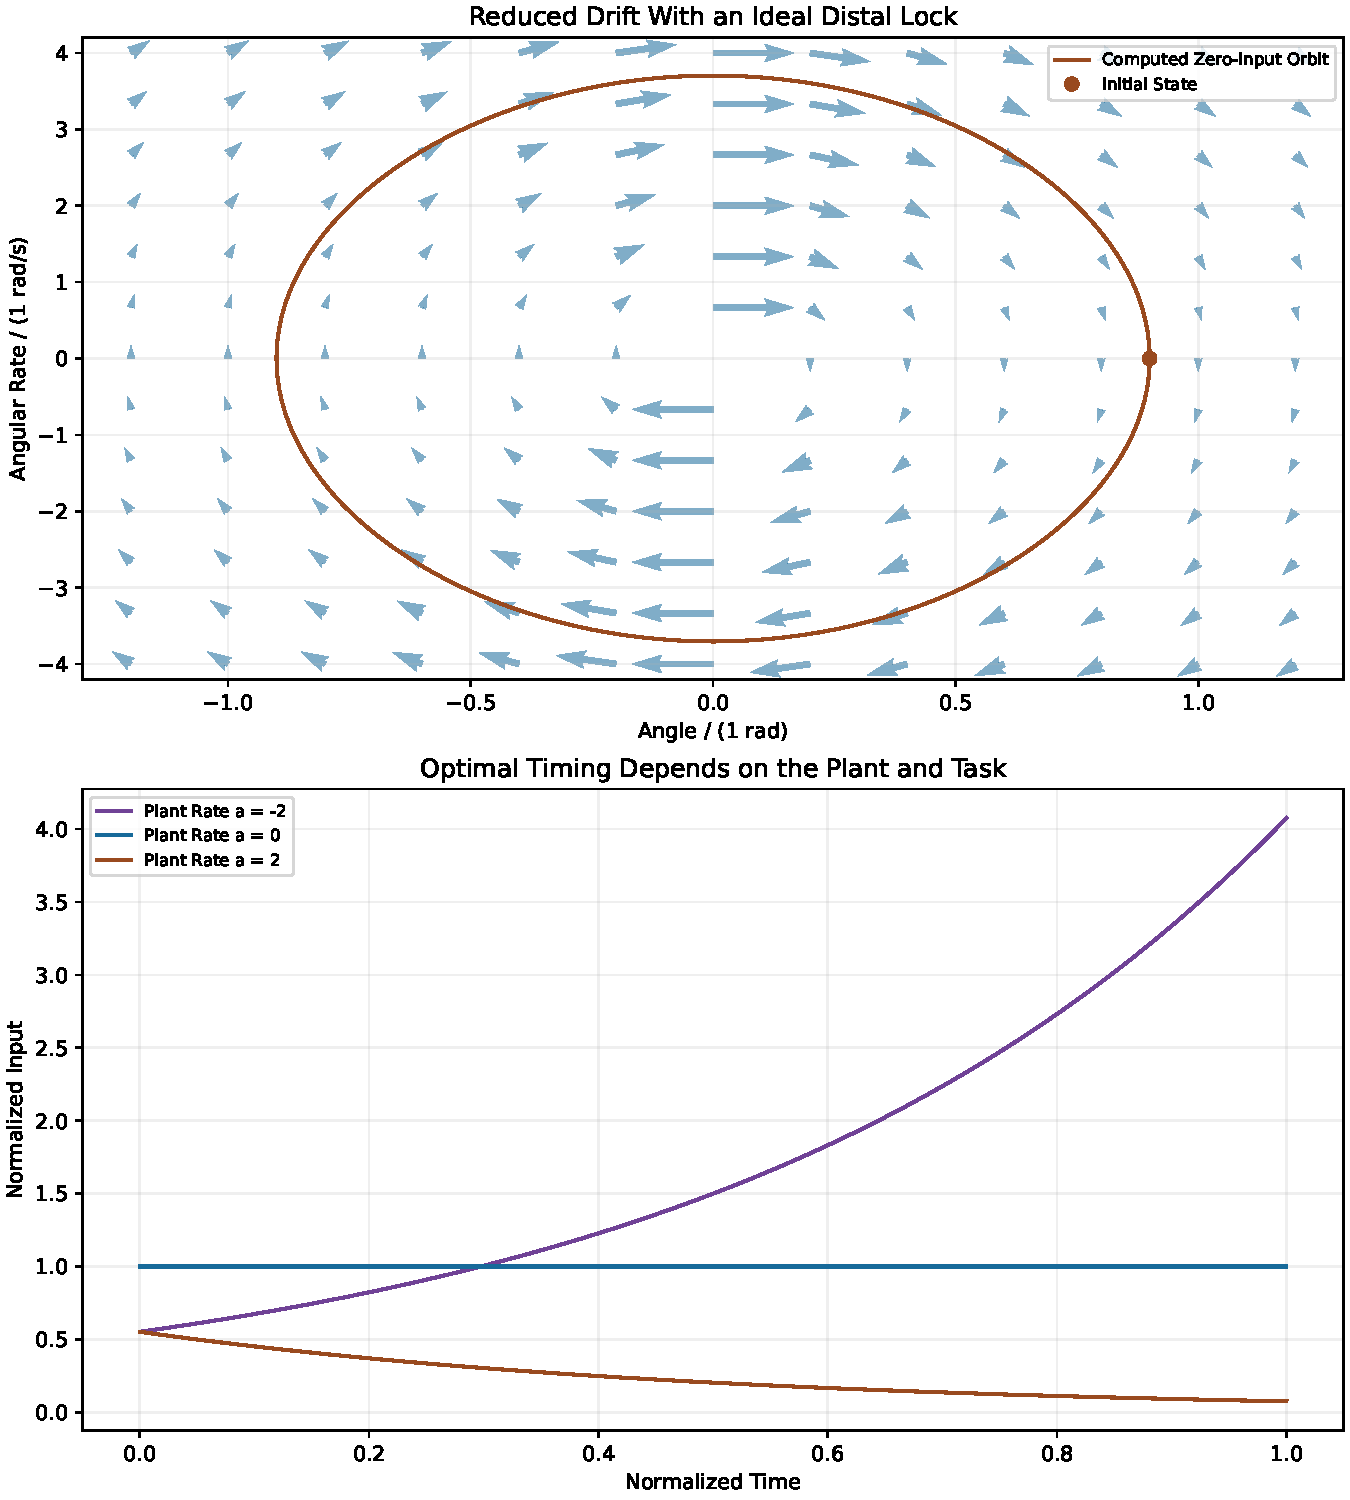
\includegraphics[width=0.9\linewidth,height=0.75\textheight,keepaspectratio]{figures/affine_structure_verified.pdf}
\caption{Declared Models of Drift and Optimal Timing. The Upper Panel Shows Normalized Directions and a Computed Orbit for the Reduced Plant With an Ideal Distal Lock. The Lower Panel Shows Exact Minimum-Energy Inputs for Three Normalized Scalar Plants With the Same Endpoint Task. Neither Panel Contains Measured Golfer Data.}
\label{fig:ch05_drift_vector_field}
\end{figure}

\subsection*{Flowing Along the Drift}
Setting an actuator torque to zero retains the declared joints and contact. Releasing a mechanical lock changes the constraints; letting go of the club removes grip forces and changes the physical system. Neither operation is represented merely by setting $u=0$ in the same fixed-pivot model. A muscle's neural drive can also become zero while activation and tendon force persist.

\begin{laymansbox}{Why Understanding Drift Matters}{box:ch05_drift_importance}
For the ideal free rigid model, $v^Tc=\tfrac12v^T\dot Mv$. Differentiating $E=T+V$ therefore gives
\[
 \dot E=v^TBu.
\]
Velocity-dependent inertial terms redistribute motion and kinetic energy within the model; they do not create mechanical energy. Gravity exchanges potential and kinetic energy. A stationary ideal constraint has zero reaction power, while moving support, damping or deformation changes the energy budget.

Acceleration, speed and power answer different questions. A force perpendicular to point velocity can bend a path without doing work. Torque can increase or decrease mechanical energy according to its power $u^TB^Tv$. A large acceleration term is not proof that its source supplied most of the energy in the swing.
\end{laymansbox}

\section{Control as a Steering Input}
Control can steer, accelerate, brake or maintain a constraint. Which effect matters depends on the input direction, configuration, velocity and task. Calling every muscular contribution ``steering'' hides its energetic role. The useful question is how an admissible change in input changes the outcome.

\subsection*{The Control Matrix as Leverage}
\begin{example}{Control Leverage at Different Configurations}{ch05_leverage}
For a perturbation $\delta u=(\delta u_1,0)^T$ with both joints free, $\delta\dot v_1=K_{11}\delta u_1$. In a coupled two-joint system,
\[
 K_{11}=\frac{1}{M_{11}-M_{12}^2/M_{22}}.
\]
The denominator is the Schur complement. If the second coordinate is held fixed instead, the proximal acceleration response is $\delta u_1/M_{11}$ and a constraint reaction supplies the required second torque. These are different experiments.

At $q_2=0$ in the manufactured example, $M_{11}=0.4205625$ kg m$^2$ and the free effective inertia is approximately $0.1128702$ kg m$^2$. Unit proximal torque produces approximately $8.860$ rad/s$^2$ of free proximal response, versus $2.378$ rad/s$^2$ with the distal coordinate locked. At $q_2=90^\circ$, the free effective inertia becomes $A=0.1505625$ kg m$^2$, so the free response is smaller, approximately $6.642$ rad/s$^2$, despite a smaller $M_{11}$. ``More folded means more leverage'' is not a general rule.

These are incremental control responses at the same state. The total acceleration also includes $a_0$, and a prescribed distal torque would add its own off-diagonal contribution. Full club acceleration additionally requires the Jacobian and its velocity-dependent term.
\end{example}

\section{The Drift-Control Ratio (DCR)}
\begin{definition}{Drift-Control Ratio}{ch05_dcr}
Specify the input origin, admissible set $\mathcal U$, state and an output/scaling map $W$. Define a capacity and a ratio by
\begin{equation}
 C_W(x)=\max_{u\in\mathcal U}\|WG(x)u\|_2,\qquad
 D_W(x)=\frac{\|Wf(x)\|_2}{C_W(x)},\quad C_W>0.
\label{eq:ch05_dcr_def}
\end{equation}
Here $W$ may select the acceleration block or normalize all derivative components using declared reference scales. Position rates and angular accelerations cannot simply be combined as unscaled numbers. A ratio using the realized input $\|WG u(t)\|$ answers a different question from a capacity ratio. Report which one is intended.

This ratio is not a work fraction, a measure of skill, or a complete reachability test. If capacity is zero, report that condition explicitly; an arbitrary epsilon changes the diagnostic and must have compatible units. Both numerator and capacity zero is indeterminate. A positive numerator with zero capacity indicates no authority through the selected map, not a finite numerical ratio.
\end{definition}

For a centered Euclidean torque ball $\|u\|_2\le u_{\max}$, $C_W=u_{\max}\sigma_{\max}(WG)$. A componentwise torque box or muscle-force polytope gives a different optimization. In particular, a 30 N m two-joint Euclidean bound does not mean both joints may independently apply 30 N m.

\begin{laymansbox}{Reading the DCR}{box:ch05_reading_dcr}
A large capacity ratio says the chosen drift norm exceeds the largest chosen control norm at that state. A small ratio says some admissible input has a larger norm; it does not show that the actual input is large or points in the useful direction. Two vectors can reinforce, oppose or be orthogonal, so their norm ratio is not an additive attribution of the observed motion.

For example, in normalized coordinates let $f=(1,0)^T$, $G=\mathrm{diag}(100,0.01)$ and $\|u\|_2\le1$. The capacity ratio is 0.01. Yet the available second-component response is at most 0.01: large first-direction authority does not help a task requiring second-direction correction. A directional capacity can instead use $\max_{u\in\mathcal U} d^TWGu$ for a declared task direction $d$.
\end{laymansbox}

A state-coordinate change $z=h(x)$ gives $f_z=Dh\,f$ and $G_z=Dh\,G$. Euclidean norms generally change. Equivalent physical comparisons require transporting the metric or the specified output; discarding different blocks after a coordinate change can define a different diagnostic. For nonlinear changes of configuration coordinates, acceleration also acquires a velocity-quadratic transformation term.

The split depends on the chosen input origin too. Under $u=u_0(x)+R(x)w$, the same dynamics become $\dot x=[f+Gu_0]+GRw$. The admissible input set must be transformed with it. The physical attainable-derivative set can remain the same while the designated drift changes. A nominal feedback policy used as a new zero input is not evidence that its energy supply became passive.

\subsection*{Address: A Defined Equilibrium}
The manufactured downward equilibrium has zero drift and nonzero torque capacity. Its capacity ratio is zero. It is equally true whether the realized torque is zero or is about to change. This does not establish a universal large torque requirement: the required torque depends on the desired acceleration and available time.

\subsection*{Top of Backswing: A Specified State}
For the manufactured state $q=(150^\circ,-70^\circ)$ and $v=0$, $a_0\simeq(-16.9466,5.2045)^T$ rad/s$^2$. With the stated 30 N m Euclidean torque bound and an unweighted angular-acceleration norm, capacity is approximately 651.113 rad/s$^2$ and the ratio is 0.02723. This is a counterexample calculation, not a measured golfer's top position or a realistic muscle-capacity estimate.

\subsection*{Downswing: Velocity Bias and Coupled Response}
At $q=(140^\circ,-60^\circ)$ and $v=(5,0)$ rad/s in the same model, $c=(0,-1.51554)^T$ N m and $g\simeq(5.57376,1.93219)^T$ N m. The complete drift acceleration is approximately $(-35.7444,42.1629)^T$ rad/s$^2$. Its capacity ratio is 0.07705. A faster state need not cross any universal threshold; geometry, velocity direction, gravity and the admissible input set all matter.

\subsection*{Impact and Beyond: Specify the Event and System}
Club-point acceleration is $\ddot p=J(q)\dot v+\dot J(q,v)v$. Its normal and tangential components are not interchangeable with joint torque. Neither 180 m/s$^2$ nor 180 times gravitational acceleration is a universal impact value; an acceleration alone cannot supply an equivalent torque without geometry and force mapping. The pre-impact smooth model does not represent the collision impulse. Contact and post-impact muscle activity require their own model and evidence.

\begin{laymansbox}{The Three Comparisons}{box:ch05_three_regimes}
Distinguish three computations: the instantaneous drift/control decomposition, the accumulated mechanical work, and the attainable change in a task before impact. Each can be useful; none substitutes for the others. Increasing a capacity ratio by reducing the torque bound makes the actuator weaker. It cannot by itself improve the best attainable outcome. Universal early/middle/late DCR categories and elite-versus-novice sensations do not follow from the equations.
\end{laymansbox}

\section{Riding the Drift: A Hypothesis to Test}
Mechanical structure can reduce the input needed for a specified task. A pendulum descending under gravity is an elementary example of exchanging stored potential for kinetic energy. But an energy-efficient movement may also require opposing drift to stop, change direction, avoid an obstacle or stabilize an unstable state. ``Align with drift'' is therefore a candidate strategy whose costs and outcomes must be calculated.

A work/power study by Nesbit and Serrano used kinematically driven full-body and club models for four amateur golfers to estimate work and energy transfer \citep{Nesbit2005b}. That scope supports distinguishing modeled joint/club work from instantaneous acceleration; it does not establish a universal DCR phase law, individual muscle activation or a globally optimal neural strategy. Net joint work is not a direct measurement of metabolic expenditure.

\section{The Geometry of the Golf Swing}
\begin{constraintbox}{The Reachability Problem}{box:ch05_reachable}
Reachability asks which states can be attained from a specified initial state over a specified time under admissible inputs and state constraints. A golf task also maps those states into club pose, velocity, impact conditions and ball outcome. Strength is one constraint, not a complete distance prediction.

If $\mathcal U_1\subseteq\mathcal U_2$ with the same plant, initial condition, horizon and other constraints, every trajectory feasible under the smaller set remains feasible under the larger. Increasing available control cannot worsen the best achievable objective under these assumptions. It does not guarantee improvement, tell a golfer which input to use, or rank technique against strength across different people.
\end{constraintbox}

Along a nominal trajectory, a smooth local model has $\delta\dot x=A(t)\delta x+B_x(t)\delta u$. At a fixed terminal time,
\[
 \delta x(T)=\Phi(T,0)\delta x(0)+\int_0^T\Phi(T,s)B_x(s)\delta u(s)\,ds.
\]
A terminal task map projects this result into the outcome. The kernel determines how an input at each time affects the task; its direction and size can change or cancel. Delay and activation restrict which inputs can occur. If impact time changes with the trajectory, event-time sensitivity must also be included. These considerations explain why an instantaneous norm ratio cannot rank early versus late control.

\section{Optimal Control and the Swing}
Specify a terminal cost $\phi$, running cost $L$, horizon and constraints:
\[
 \min_{u(\cdot)}J=\phi(x(T))+\int_0^T L(x,u,t)\,dt,\qquad
 \dot x=f(x)+G(x)u,\quad u(t)\in\mathcal U.
\]
An effort surrogate such as $u^TRu$ has declared scaling and is not mechanical power. Mechanical work integrates $u^TB^Tv$ over time; summing several torque values in N m gives neither work nor integrated effort. A model may also constrain torque rate, activation, contact, joint limits, terminal state or uncertainty. An optimizer needs all of them to define what ``best'' means.

\begin{laymansbox}{Solving the Optimal Control Problem}{box:ch05_learning}
For a smooth normal fixed-horizon problem, define the control Hamiltonian
\[
 H=L+p^T(f+Gu),\qquad \dot p=-\partial_x H,\qquad
 u^*(t)\in\arg\min_{u\in\mathcal U}H.
\]
Pontryagin's principle supplies necessary conditions, with the appropriate terminal/transversality conditions; a candidate is not automatically a global optimum. With a free terminal state, $p(T)=\nabla\phi$ in this simple formulation; terminal constraints add multipliers. This Hamiltonian is not generally mechanical energy \citep{TedrakeTrajectoryOptimality}.

Dynamic programming instead reasons about a value function. Under suitable smoothness its finite-horizon equation is $-\partial_t V=\min_u[L+\nabla_x V^T(f+Gu)]$ with terminal data $V(x,T)=\phi(x)$. Verification needs the stated boundary, admissibility and regularity conditions; nonsmooth values require more general treatment. It is not just another name for solving a single trajectory's two-point boundary-value equations \citep{TedrakeDynamicProgramming}.

Numerical solutions require feasibility, integration/discretization checks and assessment of local versus global optimality. A successful fit to a golfer's movement does not establish that the nervous system solved the optimizer or shares its cost function. Learning and feedback need independently testable predictions.
\end{laymansbox}

\begin{example}{A Solved Comparison of Control Timing}{ch05_tour_pro}
In normalized variables consider $\dot z=az+u$, $z(0)=0$, $z(1)=1$, and minimize $\int_0^1u^2dt$ with no active input bound. The endpoint condition is $1=\int_0^1e^{a(1-t)}u(t)dt$. Cauchy--Schwarz gives
\[
 J\ge\frac1{W_a},\qquad W_a=\int_0^1e^{2a(1-t)}dt,\qquad
 u^*(t)=\frac{e^{a(1-t)}}{W_a}.
\]
Equality proves the global minimum for this specified linear task. For $a=0$, $W_a=1$ and the optimal input is constant. For $a<0$, earlier effects decay and the optimal input grows toward the end. For $a>0$, earlier effects grow and the optimal input is larger early. The figure compares $a=-2,0,2$.

These plants are all control-affine. The timing follows the task sensitivity and cost, not the word ``affine'' or a universal DCR threshold. Bounds below the displayed input peaks change the solution. A golf model has more states, constraints and uncertainty; the example disproves a universal timing rule rather than prescribing a swing.
\end{example}

\section{Putting It All Together: The Unified Picture}
\subsection*{The System}
Define the body, club, supports, contacts and energy boundary before splitting forces. Drift is the zero-input derivative of that declared plant.
\subsection*{The State Space}
Include the states needed to predict force and motion: joint configuration and velocity alone may omit activation, material memory and shaft modes. Specify coordinate charts and observation uncertainty.
\subsection*{The Drift}
Prior input shaped the current state. Large present drift does not mean little past muscle work, little current energy expenditure or weak future control.
\subsection*{The Control}
The full inverse inertia, actuator mapping and admissible set determine instantaneous response. Contact and constraints can change it, while activation and delay change the time at which input is available.
\subsection*{The Skill}
A proposed strategy should predict measured task outcomes, energy costs or robustness under specified conditions. None of these is identified by an effortless feeling, a low input in one model or a large ratio alone.

\begin{principle}{Key Takeaways}{pr:ch05_key_takeaways}
Control-affine form is a precise local input structure. It makes useful calculations possible, but those calculations must still be done: complete mechanics, feasible control, energy accounting, task sensitivity and evidence. The strongest argument for exploiting mechanical structure shows how it improves a defined task under constraints. It does not require declaring muscles irrelevant or DCR the quantity every golfer should maximize.
\end{principle}



\begin{exercises}{Chapter Exercises and Worked Answers}{ex:ch05}
\subsection*{1. Compute the Declared Rest State}
For the manufactured two-link model at $q=(0,0)$, $v=0$, compute $f$. Does setting torque to zero mean releasing the club?

\textbf{Worked answer.} The bias is zero because velocity is zero, and both potential gradients vanish at downward vertical. Thus $a_0=0$ and all four components of $f$ are zero. The ideal hinges and fixed pivot remain. Releasing the club changes contact and requires a different model. Zero net torque also does not specify muscle activation or coactivation.

\subsection*{2. Compute a Raised Rest State}
Use $q=(150^\circ,-70^\circ)$ and $v=0$. Why must both gravity components enter both accelerations?

\textbf{Worked answer.} The defined potential gives $g\simeq(4.76483,1.93219)^T$ N m, and $M\simeq\left[\begin{smallmatrix}0.328445&0.153941\\0.153941&0.130000\end{smallmatrix}\right]$ kg m$^2$. Solving $Ma_0=-g$ gives $a_0\simeq(-16.9466,5.2045)^T$ rad/s$^2$. Inverse-inertia coupling mixes both loads. The first two state-derivative components remain zero at this instant even though velocity begins to change.

\subsection*{3. Separate Velocity Bias From Gravity}
For $q=(140^\circ,-60^\circ)$ and $v=(5,0)$ rad/s, compare the two acceleration contributions.

\textbf{Worked answer.} Although $v_2=0$, $c_2=b\sin(q_2)v_1^2=-1.51554$ N m. The complete contributions are $-M^{-1}c\simeq(-13.6289,28.9563)^T$ and $-M^{-1}g\simeq(-22.1155,13.2066)^T$ rad/s$^2$. Their vector sum is $(-35.7444,42.1629)^T$. Comparing only torque magnitudes or omitting $c_2$ loses the coupled response. This instantaneous decomposition is not an energy-source fraction.

\subsection*{4. Interpret a Capacity Ratio}
Use the acceleration-only norm and 30 N m Euclidean input ball for the four reported states: downward rest, $(45^\circ,0)$ at rest, raised rest, and the moving state in Exercise 3. Does the ratio identify actual muscular work?

\textbf{Worked answer.} The ratios are approximately $0$, $0.04158$, $0.02723$ and $0.07705$. They use the largest singular value of $M^{-1}$ multiplied by 30, rather than an assumed realized torque. They are not monotone in the listed angle changes and do not define golf phases. Work requires a realized torque history and the associated joint rates. Reducing the input bound increases a nonzero capacity ratio while reducing available control.

\subsection*{5. Determine Optimal Timing From a Defined Task}
For the normalized scalar endpoint problem, derive the least-energy input and determine whether early input is always preferred.

\textbf{Worked answer.} The terminal solution is $z(1)=\int_0^1e^{a(1-t)}u(t)dt$. Cauchy--Schwarz bounds its square by $W_a\int_0^1u^2dt$. Equality requires $u$ proportional to $e^{a(1-t)}$; enforcing the endpoint gives $u^*=e^{a(1-t)}/W_a$ and cost $1/W_a$. Positive, zero and negative $a$ respectively favor early, constant and late input. These are exact results for the stated normalized, unconstrained task, not a golf timing prescription.

\subsection*{6. Compare Larger and Smaller Input Sets}
If otherwise identical models have torque balls of radius 30 and 50 N m, what can be concluded about their best feasible performance and DCR?

\textbf{Worked answer.} Every 30 N m-admissible trajectory is also 50 N m-admissible. The optimum cannot become worse for the same maximization objective, or higher for the same minimization cost, when the feasible set expands. Improvement is not guaranteed. At the same state with nonzero drift, the 30 N m capacity ratio is $50/30$ times the 50 N m ratio. A larger ratio therefore cannot be a universal performance objective. Comparing different people additionally changes geometry, force capacity, coordination and uncertainty.

\subsection*{7. Compare Golf With Throwing}
What transfers from this chapter to throwing, and what must be modeled again?

\textbf{Worked answer.} A smooth torque-driven multibody phase can share the manipulator and control-affine structure. Segment geometry, actuation, constraints, initial conditions, costs and task outputs differ. Ball release changes contact and introduces event timing; golf impact adds collision mechanics. No DCR values, optimal control schedule or strength-versus-technique ranking transfers without those specifications. The same mathematical form supports different physical predictions.
\end{exercises}

\section*{Closing Thoughts: The Unity of Physics and Swing}
The affine decomposition connects a mechanical model to a control question. It is most useful when the reader can follow the entire chain: define the physical system, derive its dynamics, identify feasible inputs, propagate their effects to the task, account for energy and compare predictions with data. A simple model can reveal an important mechanism while remaining incomplete as a description of a golfer.

Induced acceleration analysis applies these mappings to specified generalized-force contributions at a given state. It must retain the same constraints and cannot infer individual muscle forces from net joint torque alone. The following chapters develop these connections; the purpose of the common framework is to make their assumptions and consequences comparable.

\flushbottom{}
